\clearpage
\begin{proofbox}
\textbf{方法一：最快证明【焦半径和差＋勾股平方差，3 步】。}

\textbf{已知：}共焦点 $F_1(-c,0),F_2(c,0)$，$a_E>c>a_H>0$。
只求右上交点 $P=(X,Y)$；其余三点由轴对称得到。

\begin{center}
% Exact model: a_E=5, c=3, a_H=2; X=10/3, Y=4 sqrt(5)/3.
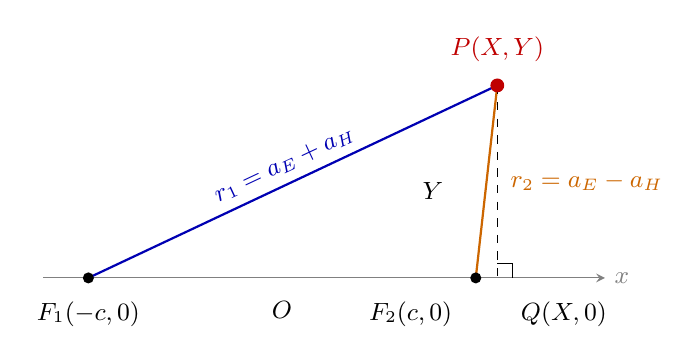
\begin{tikzpicture}[x=.82cm,y=.82cm,>=stealth,font=\small]
\coordinate (L) at (-3,0); \coordinate (R) at (3,0);
\coordinate (P) at (10/3,{4*sqrt(5)/3}); \coordinate (Q) at (10/3,0);
\draw[->,gray] (-3.7,0)--(5,0) node[right] {$x$};
\draw[blue!70!black,thick] (L)--(P) node[midway,above,sloped] {$r_1=a_E+a_H$};
\draw[orange!80!black,thick] (R)--(P) node[midway,right=5pt] {$r_2=a_E-a_H$};
\draw[dashed] (P)--(Q) node[pos=.55,left=16pt] {$Y$};
\draw (10/3,.23)--({10/3+.23},.23)--({10/3+.23},0);
\fill (L) circle (2pt) node[below=5pt] {$F_1(-c,0)$};
\fill (R) circle (2pt) node[below left=5pt] {$F_2(c,0)$};
\fill[red!75!black] (P) circle (2.5pt) node[above=5pt] {$P(X,Y)$};
\node[below right=5pt] at (Q) {$Q(X,0)$};
\node[below=5pt] at (0,0) {$O$};
\end{tikzpicture}


{\small 两条焦半径共用高度；图取 $a_E=5,c=3,a_H=2$。}
\end{center}


\textbf{第1步（两腰直接写成 $A\pm T$）。}
由椭圆、双曲线定义：
\[
PF_1+PF_2=2a_E,\quad PF_1-PF_2=2a_H
\quad\Longrightarrow\quad
PF_1=a_E+a_H,\ PF_2=a_E-a_H.
\]
\textbf{第2步（相减求 $X$）。}
勾股平方差给出
\[
4cX=PF_1^2-PF_2^2
=(a_E+a_H)^2-(a_E-a_H)^2=4a_Ea_H,
\]
故 $\displaystyle\boxed{X=a_Ea_H/c}$。

\textbf{第3步（相加求 $Y$）。}
\[
\begin{aligned}
X^2+Y^2+c^2&=\tfrac12(PF_1^2+PF_2^2)=a_E^2+a_H^2,\\
Y^2&=a_E^2+a_H^2-c^2-\frac{a_E^2a_H^2}{c^2}
=\frac{(a_E^2-c^2)(c^2-a_H^2)}{c^2}.
\end{aligned}
\]
取 $Y>0$ 即得 $Y=b_Eb_H/c$。反过来，将所得 $X^2,Y^2$ 代回：
\[
\frac{X^2}{a_E^2}+\frac{Y^2}{b_E^2}
=\frac{a_H^2+b_H^2}{c^2}=1,\qquad
\frac{X^2}{a_H^2}-\frac{Y^2}{b_H^2}
=\frac{a_E^2-b_E^2}{c^2}=1.
\]
故四种独立符号都给出交点；前面已唯一确定 $X^2,Y^2$，没有其他交点。
$0<a_H<c<a_E$ 保证 $X,Y$ 均严格为正。
\textbf{选它的理由：}只用两曲线的焦点定义、勾股定理与平方差，
不用展开或联立两条标准方程，考场最短。
\end{proofbox}

\clearpage
\begin{proofbox}
\textbf{方法二：最低门槛【从「平均值±偏差」构造交点】。}

\begin{center}
% Exact circles for a_E=4,c=2,a_H=1: radii 5 and 3, centers +/-2.
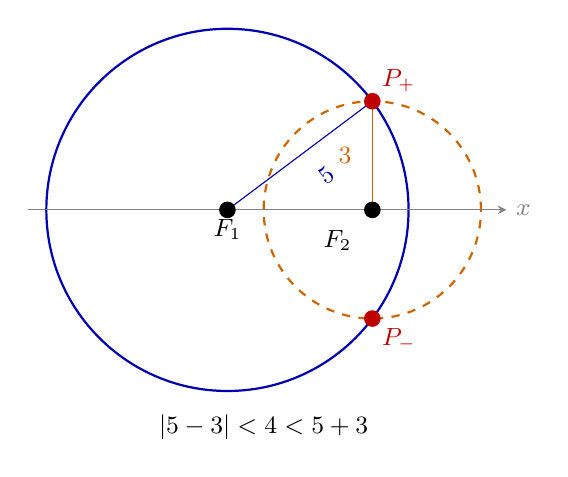
\begin{tikzpicture}[x=.46cm,y=.46cm,>=stealth,font=\small]
\draw[blue!70!black,thick] (-2,0) circle (5);
\draw[orange!80!black,thick,dashed] (2,0) circle (3);
\draw[gray,->] (-7.5,0)--(5.7,0) node[right] {$x$};
\draw[blue!70!black] (-2,0)--(2,3) node[pos=.55,below=5pt,sloped] {$5$};
\draw[orange!80!black] (2,0)--(2,3) node[midway,left=4pt] {$3$};
\fill (-2,0) circle (3pt) node[below] {$F_1$};
\fill (2,0) circle (3pt) node[below left=4pt] {$F_2$};
\fill[red!75!black] (2,3) circle (3pt) node[above right] {$P_+$};
\fill[red!75!black] (2,-3) circle (3pt) node[below right] {$P_-$};
\node at (-1,-6) {$|5-3|<4<5+3$};
\end{tikzpicture}


{\small 两个圆先确定右支上下两点，再关于 $y$ 轴反射。}
\end{center}


若学生尚不熟悉焦半径平方差，可先用初中\emph{两个距离的和与差}：
右支交点的较长距离、较短距离分别为
\[
\underbrace{a_E+a_H}_{PF_1},\qquad
\underbrace{a_E-a_H}_{PF_2}.
\]
第一步先确认\textbf{这两个圆能相交}：
以 $F_1,F_2$ 为圆心、以上述距离为半径作圆。
因为
\[
2a_H<2c<2a_E,
\]
半径之差严格小于圆心距，半径之和严格大于圆心距；
故两圆在焦点轴上下恰好交于两个点（右支上下两交点）。

第二步设上方交点 $P=(X,Y)$，从 $P$ 向焦点轴作垂线。
这时有两个初中的勾股式：
\[
(X+c)^2+Y^2=(a_E+a_H)^2,\qquad
(X-c)^2+Y^2=(a_E-a_H)^2.
\]
\textbf{为什么相减？}同一个高度 $Y$，用差便可以立即消去 $Y^2$，
求得 $X=a_Ea_H/c$。把该值代回第一个勾股式，得到
\[
Y=\sqrt{(a_E+a_H)^2-(X+c)^2}
=\frac{\sqrt{(a_E^2-c^2)(c^2-a_H^2)}}{c}.
\]
第三步在 $y$ 轴反射，得左支上下两点。
\textbf{为什么此法值得单独保留？}先证明交点确实存在，
再用熟悉的两圆相交、作高、勾股定理求位置，
把抽象「共焦二次曲线」降到初中几何。
\end{proofbox}

\clearpage
\begin{proofbox}
\textbf{方法三：常规法【两标准方程联立，按 $x^2,y^2$ 消元】。}

\begin{center}
% u=x^2,v=y^2, E: v=12-3u/4; H:v=3u-3.
\begin{tikzpicture}[x=.55cm,y=.22cm,>=stealth,font=\small]
\draw[->,gray] (-.4,0)--(17,0) node[right] {$u=x^2$};
\draw[->,gray] (0,-3.5)--(0,15) node[above] {$v=y^2$};
\draw[blue!70!black,thick] (0,12)--(16,0);
\node[blue!70!black,anchor=west] at (10,7) {$E:\ v=12-\tfrac34u$};
\draw[orange!80!black,thick,dashed] (0,-3)--(5.6,13.8);
\node[orange!80!black,right] at (5.5,13) {$H:\ v=3u-3$};
\draw[dotted] (4,0) node[below] {$4$}--(4,9)--(0,9) node[left] {$9$};
\fill[red!75!black] (4,9) circle (2.5pt) node[right=6pt] {唯一交点 $(4,9)$};
\node[anchor=west] at (7,-3) {$x=\pm2,\ y=\pm3$};
\end{tikzpicture}


{\small 例取 $a_E=4,c=2,a_H=1$；平方坐标中仅有一组正解。}
\end{center}


\[
E:\ \frac{x^2}{a_E^2}+\frac{y^2}{a_E^2-c^2}=1,
\qquad
H:\ \frac{x^2}{a_H^2}-\frac{y^2}{c^2-a_H^2}=1.
\]
\textbf{第1步：}两式都把 $y^2$ 单独写出来：
\[
\begin{aligned}
y^2&=(a_E^2-c^2)\left(1-\frac{x^2}{a_E^2}\right),\\
y^2&=(c^2-a_H^2)\left(\frac{x^2}{a_H^2}-1\right).
\end{aligned}
\]
\textbf{第2步：}令右端相等、收集 $x^2$：
\[
\begin{aligned}
a_E^2-a_H^2
&=x^2\left(\frac{a_E^2-c^2}{a_E^2}
+\frac{c^2-a_H^2}{a_H^2}\right)\\
&=x^2c^2\left(\frac1{a_H^2}-\frac1{a_E^2}\right)\\
&=x^2c^2\frac{a_E^2-a_H^2}{a_E^2a_H^2}.
\end{aligned}
\]
由于 $a_E>a_H>0$，可约去 $a_E^2-a_H^2$：
\[
\boxed{x^2=\frac{a_E^2a_H^2}{c^2}}.
\]
\textbf{第3步：}回代椭圆方程：
\[
\boxed{y^2=(a_E^2-c^2)\left(1-\frac{a_H^2}{c^2}\right)
=\frac{b_E^2b_H^2}{c^2}}.
\]
\textbf{第4步（不能省略）：}验证两个右端都严格大于 $0$，
所以 $x=\pm X$、$y=\pm Y$，且符号独立；
以上消元不存在除零、增根，四点均满足原方程。
\textbf{选它的理由：}和高中标准题的「方程联立求交点」直接对应，
也方便检查一般含参数方程。
\end{proofbox}

\clearpage
\begin{proofbox}
\textbf{方法四：补充视角【椭圆拉伸到单位圆，读出归一化位置】。}

\begin{center}
% Exact normalized coordinates u=+/-1/2,v=+/-sqrt(3)/2.
\begin{tikzpicture}[x=2.05cm,y=2.05cm,>=stealth,font=\small]
\draw[->,gray] (-1.4,0)--(1.5,0) node[right] {$u=x/a_E$};
\draw[->,gray] (0,-1.15)--(0,1.3) node[above] {$v=y/b_E$};
\draw[blue!70!black,thick] (0,0) circle (1);
\draw[orange!80!black,dashed,thick] (-.5,-1.05)--(-.5,1.05) (.5,-1.05)--(.5,1.05);
\foreach \s in {-1,1} {\foreach \t in {-1,1}
 {\fill[red!75!black] ({\s/2},{\t*sqrt(3)/2}) circle (2.3pt);}}
\node[below left] at (-.5,0) {$-\tfrac12$};
\node[below right] at (.5,0) {$\tfrac12$};
\node[above right] at (.5,{sqrt(3)/2}) {$(\tfrac12,\tfrac{\sqrt3}2)$};
\node at (0,-1.5) {$a_H/c=1/2:\quad u=\pm1/2$};
\end{tikzpicture}


{\small 单位圆上两条竖线，各截出上下两点。}
\end{center}


设 $u=x/a_E$、$v=y/b_E$，则椭圆成为 $u^2+v^2=1$。
由双曲线方程
\[
\frac{a_E^2u^2}{a_H^2}-\frac{b_E^2v^2}{b_H^2}=1.
\]
再利用 $v^2=1-u^2$，有
\[
u^2\left(\frac{a_E^2}{a_H^2}+\frac{b_E^2}{b_H^2}\right)
=1+\frac{b_E^2}{b_H^2}.
\]
左右分别整理（$b_E^2=a_E^2-c^2$，$b_H^2=c^2-a_H^2$），
得到 $u^2=a_H^2/c^2$、$v^2=b_H^2/c^2$。
因为 $u^2+v^2=1$，这正是单位圆上\emph{两条竖直线}
$u=\pm a_H/c$ 与圆的四个交点。
还原缩放 $x=a_Eu,y=b_Ev$，立即得到 $x=\pm a_Ea_H/c$、
$y=\pm b_Eb_H/c$。
\textbf{保留理由：}联系「椭圆是圆的非等比缩放」，
便于理解两个曲线参数如何共同决定交点位置。
\end{proofbox}

\clearpage
\begin{proofbox}
\textbf{推论证明：四交点切线正交（两种可选证明）。}

\textbf{证明 A：最快斜率法。}

\begin{center}
% At P=(2,3), slopes -1/2 and 2. Same scale on both axes.
\begin{tikzpicture}[x=.75cm,y=.75cm,>=stealth,font=\small]
\draw[->,gray] (-2.7,0)--(5.6,0) node[right] {$x$};
\draw[blue!70!black,thick,domain=15:105,samples=70,variable=\t]
 plot ({4*cos(\t)},{sqrt(12)*sin(\t)});
\draw[orange!80!black,thick,domain=.3:4.9,samples=70,variable=\t]
 plot ({sqrt(1+\t*\t/3)},\t);
\draw[blue!70!black,dashed] (-.5,4.25)--(5.2,1.4) node[right] {$k_E=-1/2$};
\draw[orange!80!black,dashed] (.6,.2)--(3,5) node[above right] {$k_H=2$};
\draw[gray] (-2,0)--(2,3)--(2,0);
\draw[thick] (2.358,2.821)--(2.537,3.179)--(2.179,3.358);
\fill[red!75!black] (2,3) circle (2.5pt) node[above left=5pt] {$P$};
\fill (-2,0) circle (2pt) node[below] {$F_1$};
\fill (2,0) circle (2pt) node[below] {$F_2$};
\node at (0,-1.3) {切线夹角 $90^\circ$，焦角 $\cos\theta=3/5$};
\end{tikzpicture}


{\small 实线为曲线，虚线为交点处切线；两轴比例相同。}
\end{center}

椭圆、双曲线在交点的切线斜率分别为
\[
k_E=-\frac{b_E^2x}{a_E^2y},\qquad
k_H=\frac{b_H^2x}{a_H^2y}.
\]
交点坐标平方代入便得
\[
k_Ek_H=-\frac{b_E^2b_H^2}{a_E^2a_H^2}
\frac{x^2}{y^2}=-1.
\]

\end{proofbox}
\clearpage
\begin{proofbox}
\textbf{证明 B：焦点定义的梯度向量法（教师可选）。}

\begin{center}
% u=(4/5,3/5), v=(0,1): both unit length; sum=(.8,1.6), diff=(.8,-.4).
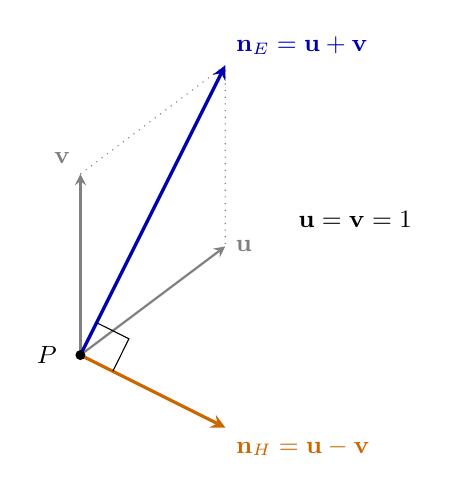
\begin{tikzpicture}[x=2.3cm,y=2.3cm,>=stealth,font=\small]
\coordinate (P) at (0,0);
\draw[gray,dotted] (0,1)--(.8,1.6)--(.8,.6);
\draw[->,gray,thick] (P)--(.8,.6) node[right] {$\mathbf u$};
\draw[->,gray,thick] (P)--(0,1) node[above left] {$\mathbf v$};
\draw[->,blue!70!black,very thick] (P)--(.8,1.6) node[above right] {$\mathbf n_E=\mathbf u+\mathbf v$};
\draw[->,orange!80!black,very thick] (P)--(.8,-.4) node[below right] {$\mathbf n_H=\mathbf u-\mathbf v$};
\draw (.089,.179)--(.268,.09)--(.179,-.089);
\fill (P) circle (1.8pt) node[left=5pt] {$P$};
\node[anchor=west] at (1.15,.75) {$\lVert\mathbf u\rVert=\lVert\mathbf v\rVert=1$};
\end{tikzpicture}


{\small 两单位向量的和、差垂直；箭头统一从 $P$ 出发。}
\end{center}

记从两焦点指向交点 $P$ 的单位向量为
$\mathbf u=(P-F_1)/PF_1$、$\mathbf v=(P-F_2)/PF_2$。
椭圆「距离和」的法向量为 $\mathbf u+\mathbf v$，
双曲线「距离差」的法向量为 $\mathbf u-\mathbf v$
（左支只差一个整体负号）。
于是
\[
(\mathbf u+\mathbf v)\cdot(\mathbf u-\mathbf v)
=\lVert\mathbf u\rVert^2-\lVert\mathbf v\rVert^2=0.
\]
两法线垂直，因此两切线也垂直。
\textbf{说明：}这条推论是 C094 的几何扩展，不能拿它代替
C090 的焦点张角 $\angle F_1PF_2$。
\end{proofbox}
